% !TEX root = ../lab1.tex
\section{Техническое задание}

\begin{itemize}
	\item Подобрать некачественное (засвеченное) изображение в цветовом формате RGB;
	\item Преобразовать его при помощи математического алгоритма в черно-белый формат;
	\item Получить цветовую гистограмму изображения;
	\item При помощи методов улучшения гистограмм получить более качественные изображения в черно-белом формате.
\end{itemize}

\section{Ход работы}

Для выполнения работы был разработан класс ShadeFix с использованием библиотек OpenCV и Matplotlib на языке Python (листинг \vref{lst:shadefix}). Пример его использования приведен в листинге \cref{lst:mainpy}, а использованные зависимости для virtualenv --- в листинге \cref{lst:requirements}.

\subsection{Преобразование цветного изображения в черно-белое}

Исходное изображение представлено на \vref{pic:test}.

\begin{figure}[H]
	\centering
	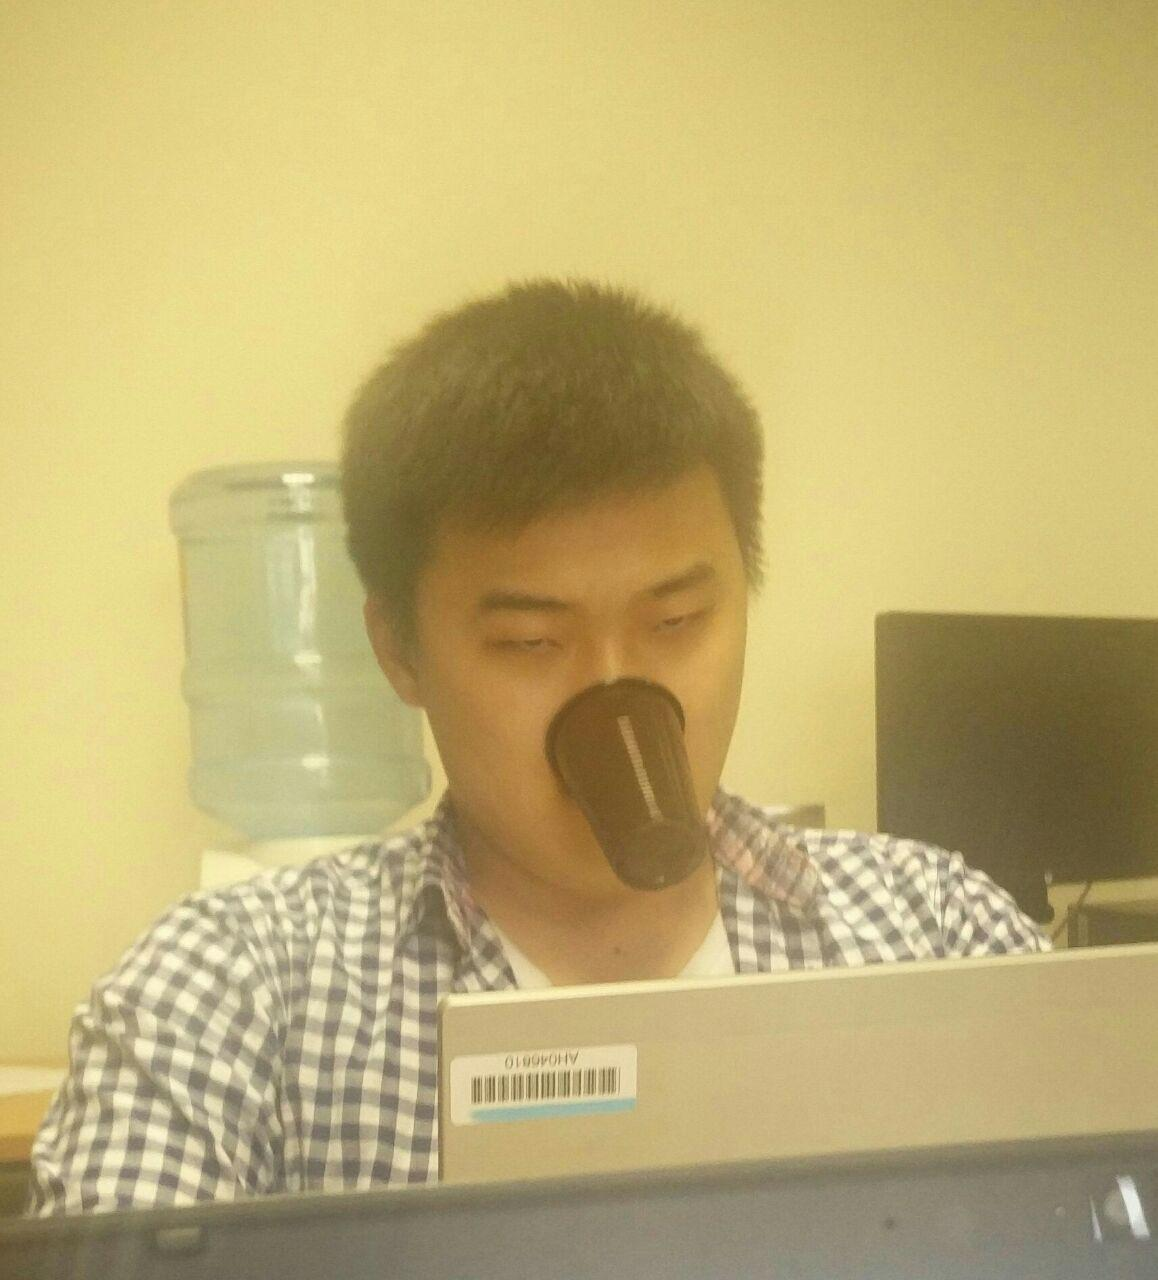
\includegraphics[width=0.50\textwidth]{test}
	\caption{Некачественно цветное изображение в формате RGB}
	\label{pic:test}
\end{figure}

Для преобразования цветного изображения в черно-белое воспользуемся формулой \vref{eq:gray}.

\begin{equation} \label{eq:gray}
	Gray_{x,y} = 0.299 \times R_{x,y} + 0.587 \times G_{x,y} + 0.114 \times B_{x,y}
\end{equation}

В классе ShadeFix преобразование выполняется с помощью метода \texttt{toGreyscale}.

На \vref{pic:grey1} показано изображение, полученное в результате работы программы.

\begin{figure}[H]
	\centering
	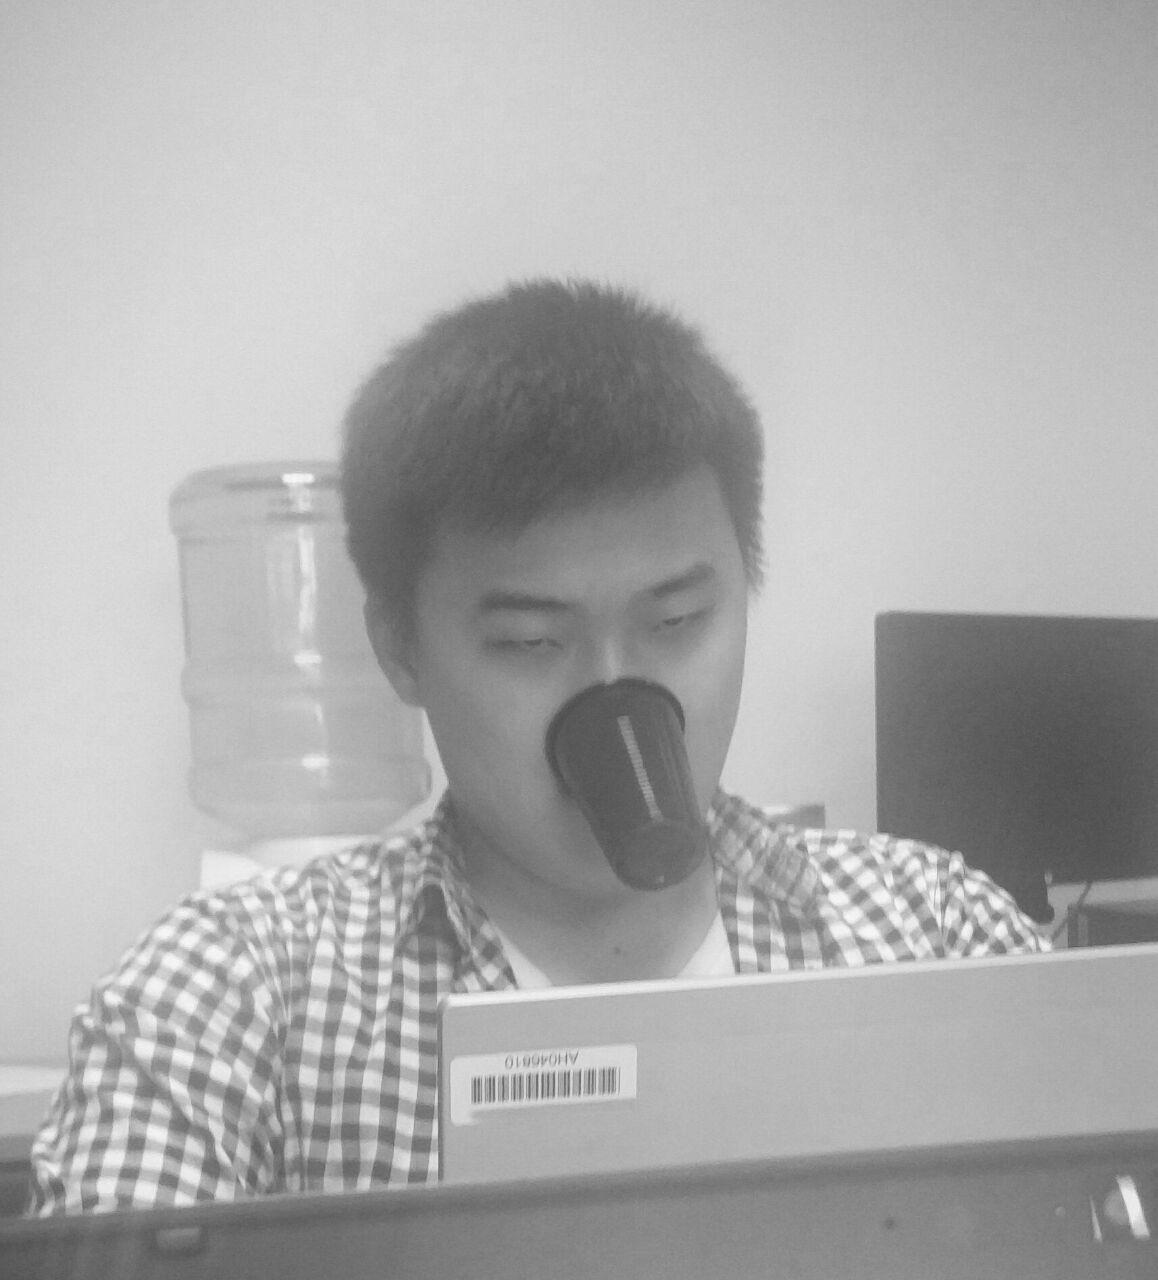
\includegraphics[width=0.50\textwidth]{grey1}
	\caption{Черно-белое изображение, полученное в результате работы программы}
	\label{pic:grey1}
\end{figure}

Для построения гистограммы изображения используется метод \texttt{makeHistogram}.

Гистограмма полученного изображения представлена на \vref{pic:hist1}.

\begin{figure}[H]
	\centering
	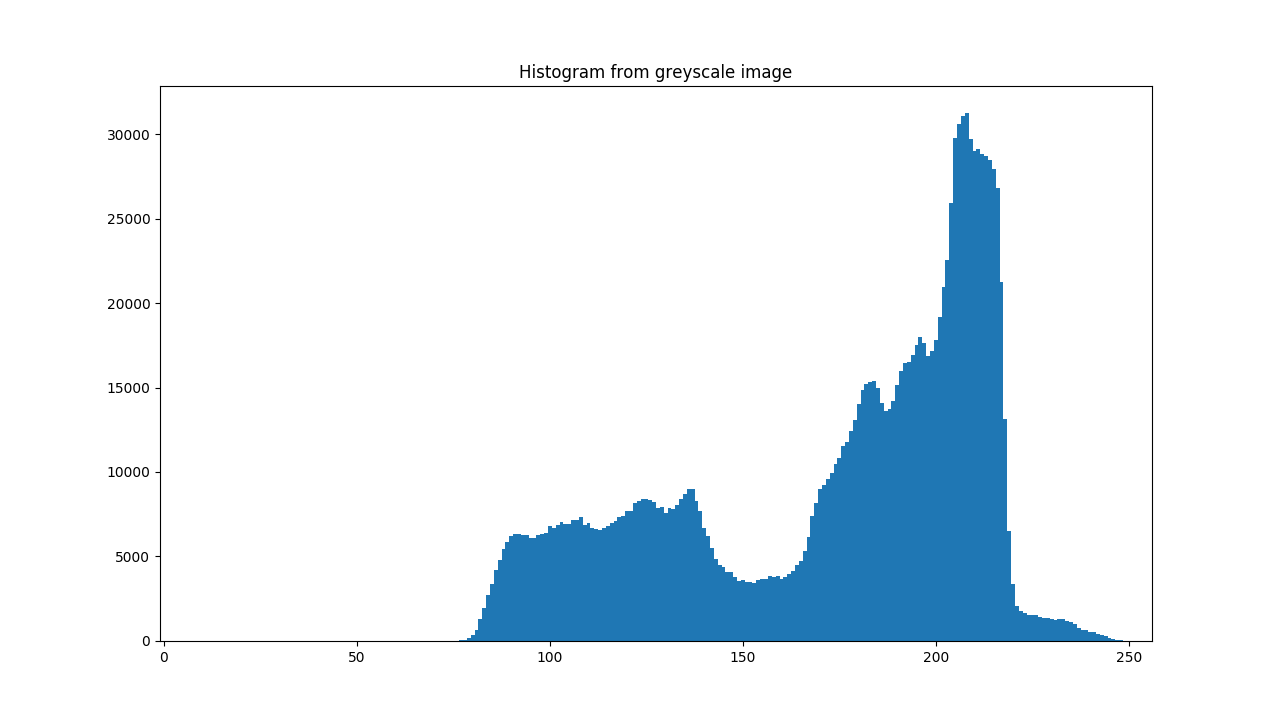
\includegraphics[width=\textwidth]{hist1}
	\caption{Исходная гистограмма черно-белого изображения}
	\label{pic:hist1}
\end{figure}

\subsection{Линейное растяжение гистограммы изображения}

При выполнении линейного растяжения пренебрежем малыми цветами (порог 5\%). Для этого используется метод \texttt{normalizeShadeMap}. Результирующая гистограмма представлена на \vref{pic:hist2}.

\begin{figure}[H]
	\centering
	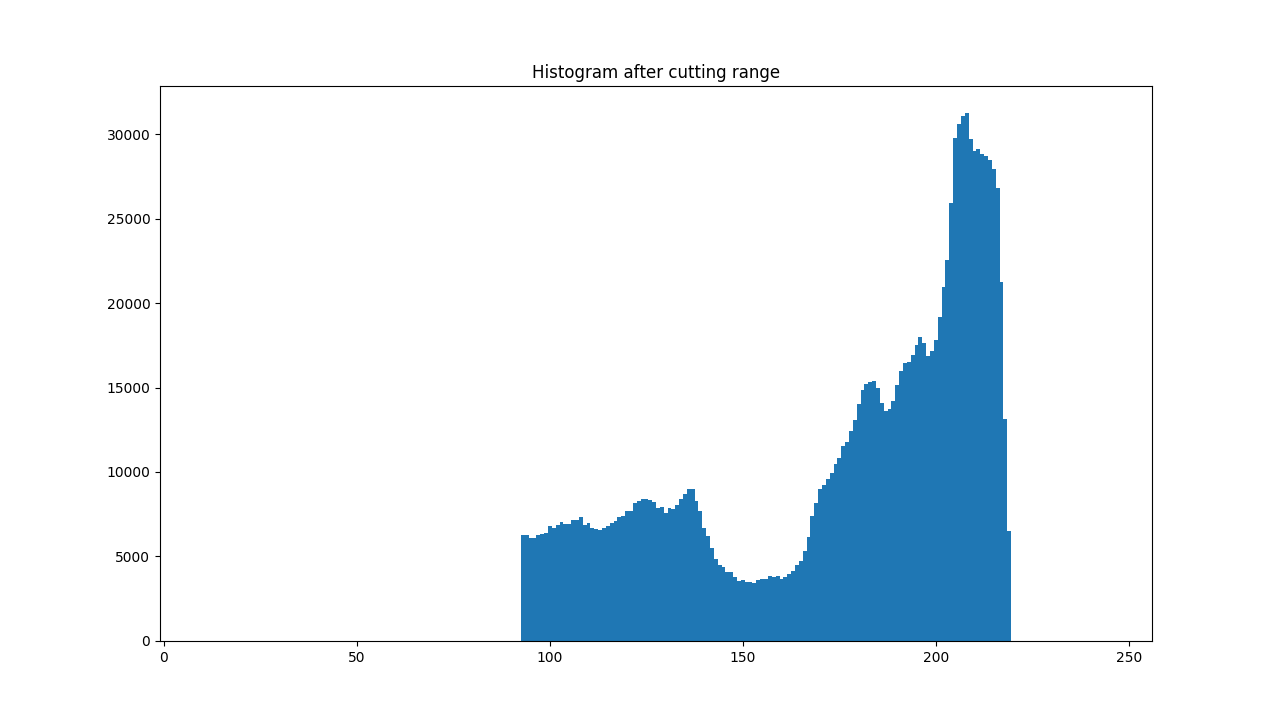
\includegraphics[width=\textwidth]{hist2}
	\caption{Результирующая гистограмма черно-белого изображения}
	\label{pic:hist2}
\end{figure}

Улучшим качество изображения с помощью метода линейного растяжения. Для этого воспользуемся формулой \vref{eq:ls}, где $f_{x,y}^{out}$ --- значение оттенка нового пикселя, $f_{x,y}^{in}$ --- значение оттенка старого пикселя, $a$ и $b$ --- нижний и верхний границы гистограммы, $c$ и $d$ --- новые границы гистограммы. В классе ShadeFix данная формула реализована в методе \texttt{linearStretching}.

\begin{equation} \label{eq:ls}
	f_{x,y}^{out}=(f_{x,y}^{in}-a)*\frac{d-c}{b-a}+c
\end{equation}

Полученная в результате данного преобразования гистограмма приведена на \vref{pic:hist3}, а результирующее изображение --- на \vref{pic:grey2}.

\begin{figure}[H]
	\centering
	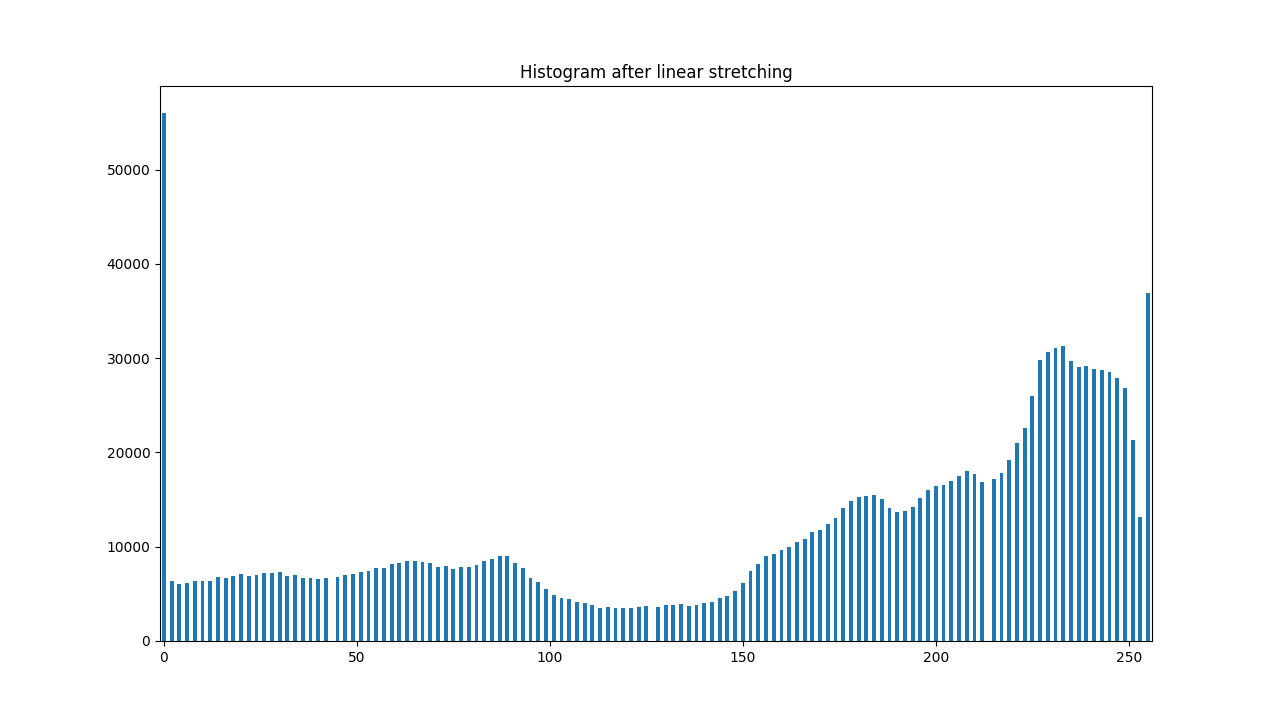
\includegraphics[width=\textwidth]{hist3}
	\caption{Гистограмма с применением метода линейного растяжения}
	\label{pic:hist3}
\end{figure}

\begin{figure}[H]
	\centering
	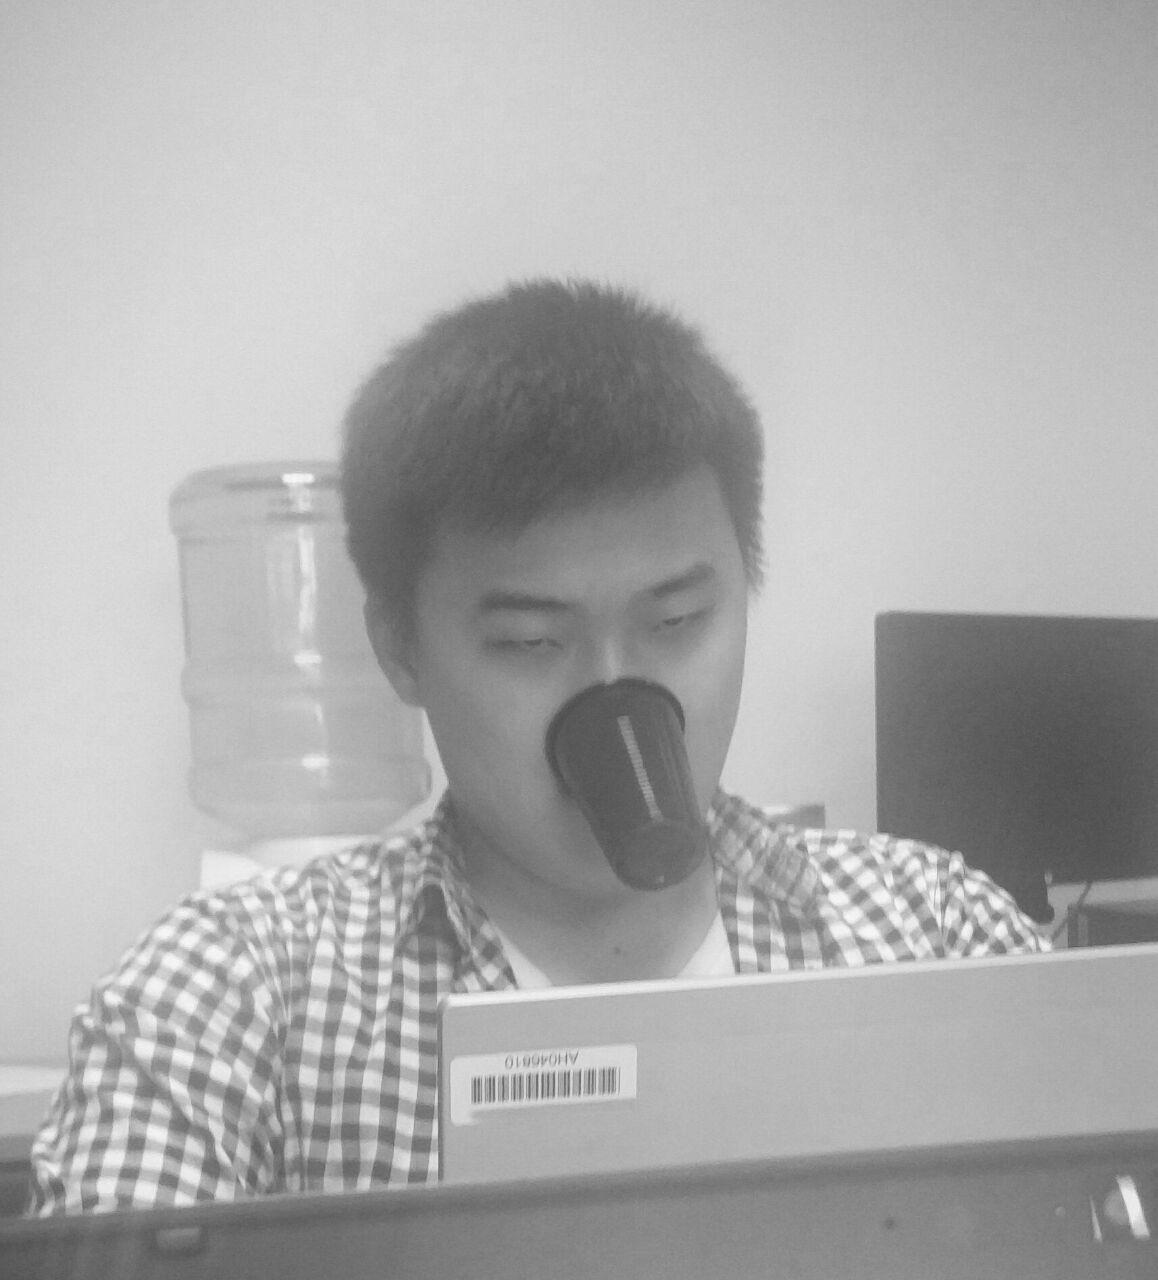
\includegraphics[width=0.45\textwidth]{grey1}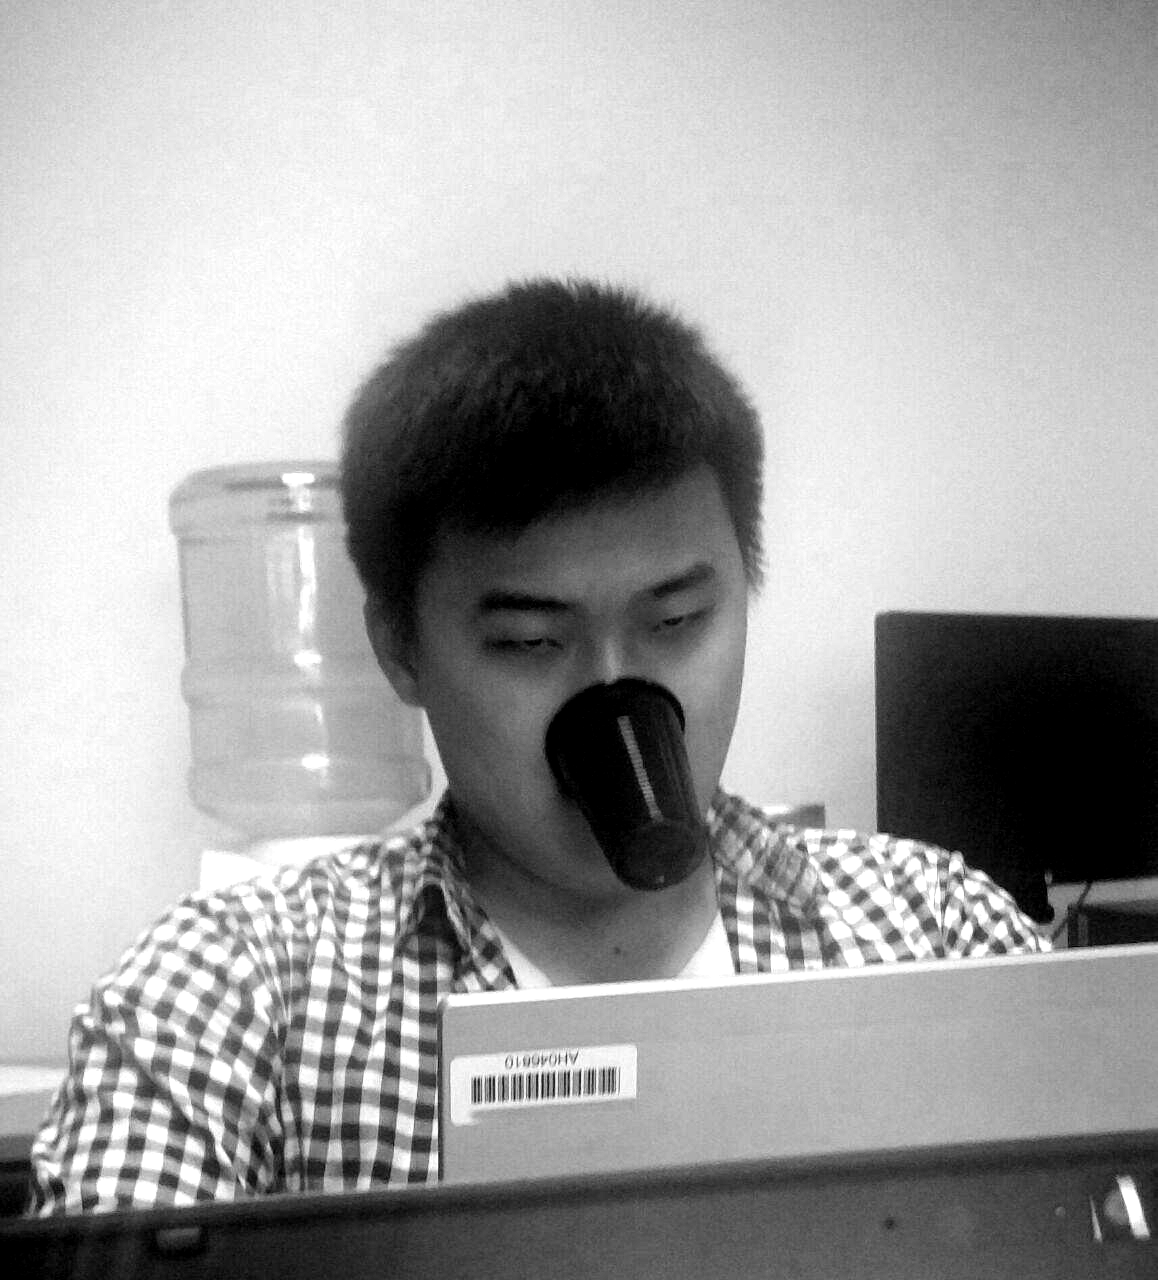
\includegraphics[width=0.45\textwidth]{grey2}
	\caption{Изображение, полученное в ходе растяжения гистограммы (справа), в сравнении с исходным}
	\label{pic:grey2}
\end{figure}

\subsection{Эквализация гистограммы изображения}

Попробуем улучшить исходное изображение путем эквализации его гистограммы. Для этого воспользуемся формулой \vref{eq:he}, где $S_k$ --- элемент LookUp таблицы (хранящий новые значения оттенков для замены старых), $n_j$ --- число пикселей с оттенком $j$, $n$ --- число всех пикселей.  В классе ShadeFix данная формула реализована в методе \texttt{histogramEqualization}.

\begin{equation} \label{eq:he}
	S_k=\sum_{j=0}^{k}\frac{n_j}{n}
\end{equation}

Полученная в результате данного преобразования гистограмма приведена на \cref{pic:hist4}, а результирующее изображение --- на \vref{pic:grey3}.

\begin{figure}[H]
	\centering
	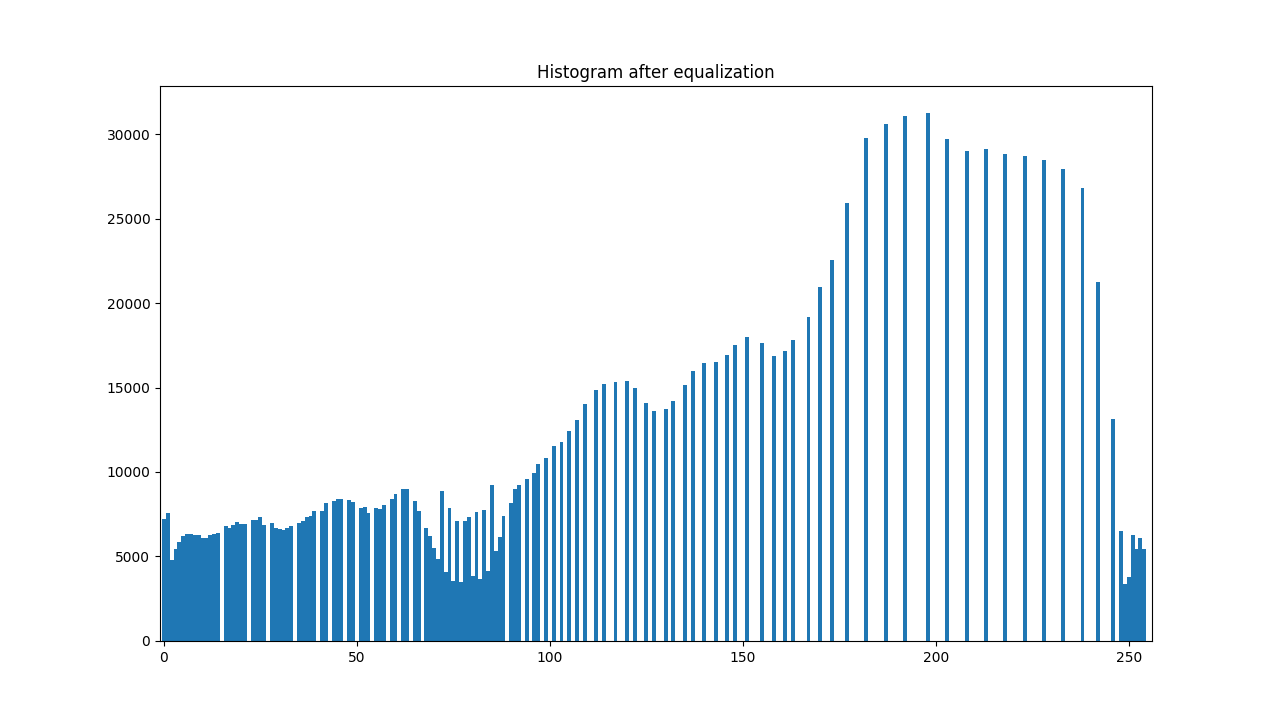
\includegraphics[width=\textwidth]{hist4}
	\caption{Гистограмма с применением метода эквализации гистограммы}
	\label{pic:hist4}
\end{figure}

\begin{figure}[H]
	\centering
	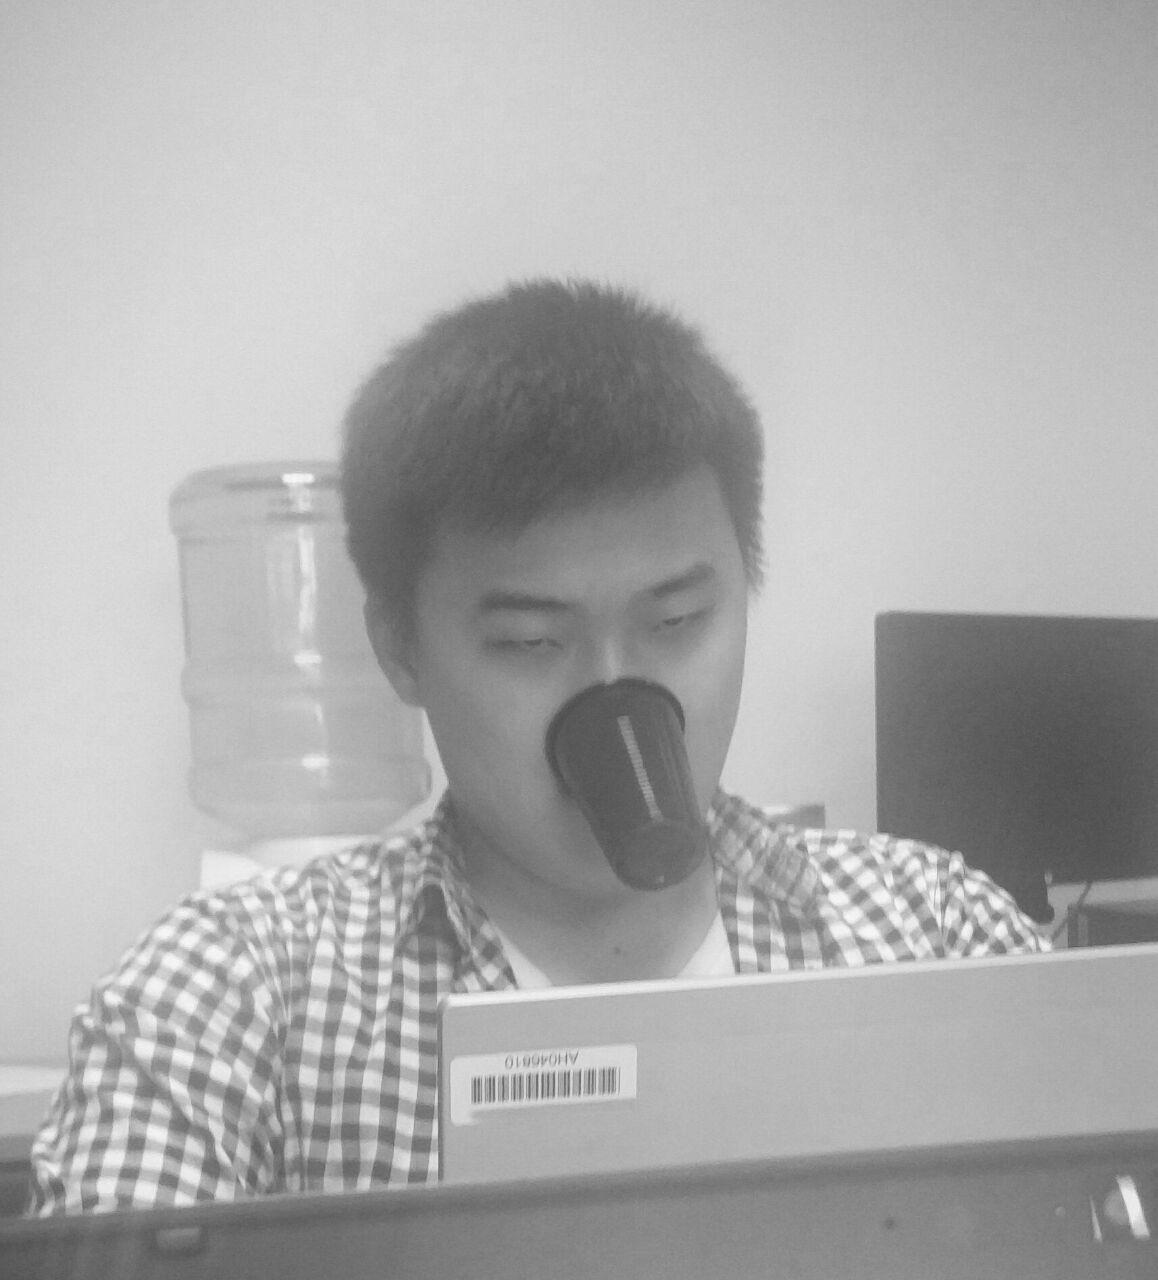
\includegraphics[width=0.45\textwidth]{grey1}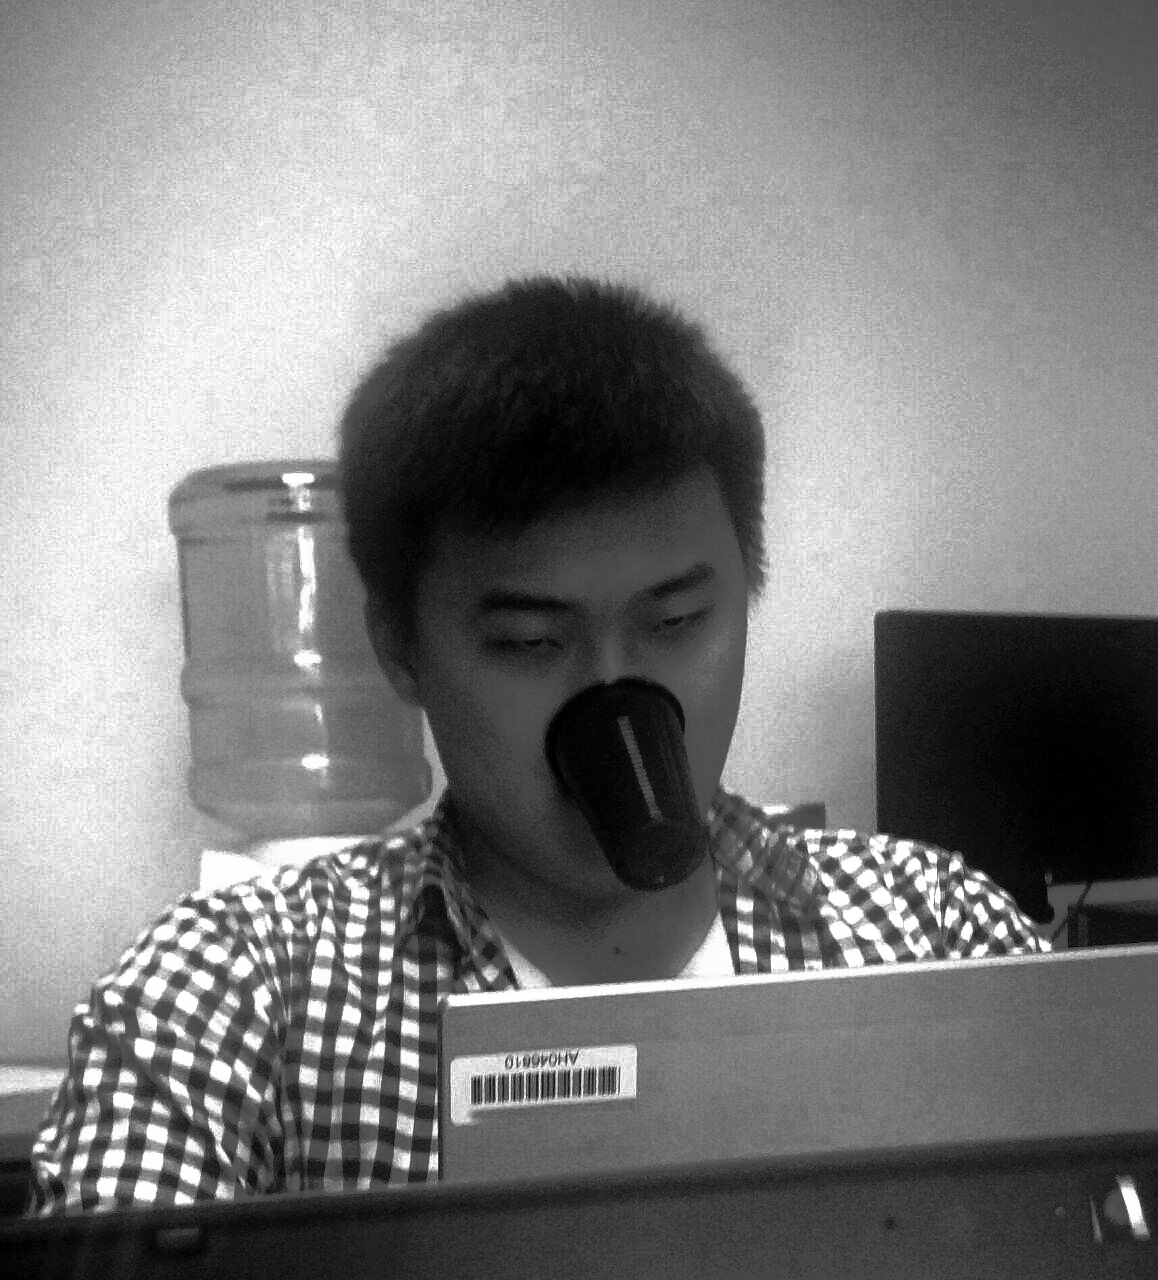
\includegraphics[width=0.45\textwidth]{grey3}
	\caption{Изображение, полученное в ходе эквализации гистограммы (справа), в сравнении с исходным}
	\label{pic:grey3}
\end{figure}

\section{Выводы}

В ходе данной работы был разработан класс для улучшения засвеченного черно-белого изображения с помощью методов линейного растяжения и эквализации гистограммы.

При исследовании гистограмм после линейного растяжения и эквализации гистограммы можно заметить, что метод линейного растяжения "`растягивает"' исходную гистограмму на весь диапазон оттенков, а метод эквализации гистограммы старается обеспечить средний уровень количества пикселей по всей гистограмме (так, в случае, когда на один оттенок приходится большое количество пикселей, расстояние до соседних ненулевых оттенков сравнимо больше, чем в случае оттенка с малым числом пикселей).

В результате выполнения работы было обнаружено, что линейное растяжение неплохо уменьшает засвеченность изображения, однако для этого необходимо, чтобы в гистограмме отсутствовали оттенки на ее границах (в данном случае 0 и 255), поскольку в таком случае действенность этого метода резко ухудшается. Эквализация гистограммы же может привести к сильному затемнению или засветлению изображения (создать "`шумы"'). Обычно подобный эффект проявляется на почти однотонных участках исходного изображения (из близких оттенков). Вызвана данная ситуация перераспределением пикселей, обеспечивающих плавный переход, к разным контрастным оттенкам (наблюдаемые на результирующей гистограмме расстояния между соседними ненулевыми оттенками), что приводит к увеличению контрастности и ухудшению плавности. 